\documentclass{llncs}

\usepackage[utf8]{inputenc}
\usepackage{amsmath}
\usepackage{amssymb}
\usepackage{amsfonts}
\usepackage{graphicx}
\usepackage{graphicx}
\usepackage[justification=centering]{caption}
\usepackage{pdflscape}
\usepackage{multicol}
\usepackage{subfig}
\usepackage{xspace}

\usepackage{bussproofs}
\usepackage{proof}
\usepackage{url}

\usepackage{fancybox}
\usepackage{fancyvrb}

% Sequent Calculus Proof Settings
\EnableBpAbbreviations
\def\fCenter{\mbox{\ $\vdash$\ }}
\newcommand{\rl}[1]{\RightLabel{#1}}

\usepackage{commands}

\newif\ifcomments
\commentstrue
%\commentsfalse   % gobble comments, set for final version

\ifcomments
  \newcommand{\paf}[1]{\par\noindent{\sf PF: #1}\par\medskip}
  \newcommand{\dd}[1]{\par\noindent{\sf DD: #1}\par\medskip}
  \newcommand{\bw}[1]{\par\noindent{\sf BW: #1}\par\medskip}
  \newcommand{\sm}[1]{\par\noindent{\sf SM: #1}\par\medskip}
  \newcommand{\PAF}[1]{\marginpar{\footnotesize{\sf PF: #1}}}
  \newcommand{\DD}[1]{\marginpar{\footnotesize{\sf DD: #1}}}
  \newcommand{\BW}[1]{\marginpar{\footnotesize{\sf BW: #1}}}
  \newcommand{\SM}[1]{\marginpar{\footnotesize{\sf SM: #1}}}
\else
  \newcommand{\paf}[1]{}
  \newcommand{\dd}[1]{}
  \newcommand{\bw}[1]{}
  \newcommand{\sm}[1]{}
  \newcommand{\PAF}[1]{}
  \newcommand{\DD}[1]{}
  \newcommand{\BW}[1]{}
  \newcommand{\SM}[1]{}
\fi


\title{
  Implementation and Evaluation of \\ 
  Contextual Natural Deduction \\
  for Minimal Logic
}

\author{
  Bruno Woltzenlogel Paleo\thanks{Stipendiat der \"Osterreichischen Akademie der Wissenschaften (APART).}%\inst{1,2}
}

\authorrunning{B.\~Woltzenlogel Paleo}

\institute{
  Vienna University of Technology \\
  Australian National University \\
  \email{bruno.wp@gmail.com}
}

% ===========================================================================



\newcommand{\RPlong}{\texttt{RecyclePivots}}
\newcommand{\RPIlong}{\texttt{RecyclePivotsWithIntersection}}
\newcommand{\LUlong}{\texttt{LowerUnits}}

\newcommand{\RP}{\texttt{RP}}
\newcommand{\RPI}{\texttt{RPI}}
\newcommand{\LU}{\texttt{LU}}

\newcommand{\VeriT}{\texttt{VeriT}\xspace}
\newcommand{\Skeptik}{\texttt{Skeptik}\xspace}


\newenvironment{calculus}
{\begin{center}\begin{Sbox}\begin{minipage}{0.9\textwidth}}
{\end{minipage}\end{Sbox}\fbox{\TheSbox}\end{center}}


\newcommand{\tP}[1]{\xi[#1]}
\newcommand{\tN}[1]{\zeta[#1]}
\newcommand{\eS}{\epsilon}

\newcommand{\AtPosition}{\textrm{At}}

\renewcommand{\defEq}{=}

% ===========================================================================

\begin{document}

\maketitle

\newcommand{\ND}{$\textbf{ND}$\xspace}
\newcommand{\NDd}{$\textbf{ND}^\textbf{c}$\xspace}
\newcommand{\lc}{\lambda^c}

\begin{abstract}
The \emph{contextual} natural deduction calculus ({\NDd}) extends the usual natural deduction calculus ({\ND}) by allowing the implication introduction and elimination rules to operate on formulas that occur inside contexts. It has been shown that, asymptotically in the best case, {\NDd}-proofs can be quadratically smaller than the smallest {\ND}-proofs of the same theorems. In this paper we describe the first implementation of a theorem prover for minimal logic based on {\NDd}. Furthermore, we empirically compare it to an equally simple {\ND} theorem prover on thousands of randomly generated conjectures.
\end{abstract}


\section{Introduction}

\emph{Natural deduction} was introduced by Gentzen in \cite{Gentzen1934Untersuchungen-uber-das-logische-Schliesen} and one of its distinguishing features is that the meaning of a logical connective is determined by elimination and introduction rules, and not by axioms. As a result, formal natural deduction proofs are considered to be similar in structure to their informal counterparts and hence more \emph{natural}. This subjective claim is corroborated by the observation that widely used proof assistants\footnote{e.g. Isabelle {\scriptsize (\url{www.cl.cam.ac.uk/research/hvg/Isabelle/})} and Coq {\scriptsize (\url{http://coq.inria.fr})}.} 
follow a natural deduction style.

However, as exemplified in \cite{NDc}, the inference rules of natural deduction style calculi can be inconvenient, lengthy and ultimately unnatural for formalizing reasoning steps that modify a deeply located subformula of a formula, such as: Tseitin's transformation, skolemization, double negation elimination, quantifier shifting, prenexification\ldots  \ Because these deep reasoning steps are commonly used by automated deduction tools during preprocessing of the theorem to be proved, the resulting proofs may contain deep inferences \cite{DeharbeFontaineWoltzenlogel-Paleo2011Quantifier-Inference-Rules-in-the-Proof-Format-of-VeriT}. Therefore, automatically replaying (i.e. reproving) these proofs in proof assistants (e.g. when an automated deduction tool is integrated within a proof assistant \cite{BohmeNipkow2010Sledgehammer:-Judgement-Day}) can be inefficient in terms of proving time and size of the generated shallow proof.

These challenges motivated the invention (in \cite{NDc}) of the \emph{contextual natural deduction calculus} (\NDd), which is a simple extension of the usual natural deduction calculus (here called {\ND}) allowing introduction and elimination rules to operate on formulas occurring inside contexts. The goals in \cite{NDc} were purely theoretical. It was shown that {\NDd} is sound and complete, that proofs can be normalized, and that some proofs can be quadratically smaller than the smallest proofs of the same theorem in the usual natural deduction calculus. In contrast, the main goal of the work reported in the present paper is to evaluate {\NDd} empirically. This is important, because asymptotic proof-complexity results can be misleading when the assymptotic behaviour they describe for particular worst cases or best cases is not observed in cases that occur most often in practice.

{\NDd} can be regarded not only from a theorem proving perspective but also from a \emph{proof compression} point of view: a given {\ND}-proof $\psi$ could be compressed by transforming it to a smaller {\NDd}-proof. Since every {\ND}-proof is also an {\NDd}-proof, a straightforward proof compression algorithm could simply try to reprove $\psi$'s theorem using an {\NDd} theorem prover.

The implementation of prototypical theorem provers based on {\ND} and {\NDd} within the {\Skeptik} framework (\url{github.com/Paradoxika/Skeptik}) %\cite{SkeptikSystemDescription}
is discussed in Section \ref{sec:Implementation}. These provers are restricted to minimal logic (intuitionistic logic having only the implication connective). Although it would be straightforward to extend the contextual techniques to inference rules for other connectives as well, the restriction to minimal logic implies less implementation effort and is sufficient to estimate how promising the idea of contextual natural deduction might be in practice. An experimental infra-structure, including a random formula generator, also had to be implemented, as briefly described in Section \ref{sec:ExperimentalSetup}. The experimental results are shown and analyzed in Section \ref{sec:Results}.


\medskip

\noindent\textbf{Related work:} due to the increasing maturity of automated deduction tools, there has been a lot of recent work on proof production~\cite{APPABook} and on the development of algorithms for simplifying the generated proofs in a post-processing phase. These methods have focused mostly on propositional resolution proofs output by SAT- and SMT-solvers so far~\cite{RP,RPILU,LUniv,RedRec,Split,Skeptik}, 
but generalizations to first-order resolution have been proposed as well~\cite{FOLU}. 
There are also algorithms aimed at compressing and structuring sequent calculus proofs by eliminating or introducing cuts \cite{Woltzenlogel-Paleo2010Atomic-Cut-Introduction-by-Resolution:-Proof-Structuring-and-Compression,HetzlLeitschWeller2012Towards-Algorithmic-Cut-Introduction,RedundancyInCutElimination,PhDThesis} or by extracting Herbrand sequents from proofs \cite{HerbrandSequent,HerbrandSequentThesis,HerbrandSequentBook}. 
\cite{NDc} is probably the first work considering, from a theoretical perspective, the compressibility of natural deduction proofs, and this paper reports the first realization of this idea in practice. Contextual inferences have a lot in common with the related idea of \emph{deep inference}, which has been intensively investigated in the last decade, especially for classical logic (e.g. \cite{Brunnler2003Atomic-Cut-Elimination-for-classical-Logic,BruscoliGuglielmiGundersenParigot2010A-Quasipolynomial-Cut-Elimination-Procedure-in-Deep-Inference-via-Atomic-Flows-and-Threshold-Formulae,BruscoliGuglielmi2009On-the-Proof-Complexity-of-Deep-Inference,Guglielmi1999A-System-of-Interaction-and-Structure}) but also for intuitionistic logic \cite{Tiu2006A-Local-System-for-Intuitionistic-Logic,BruennlerMcKinley2008An-Algorithmic-Interpretation-of-a-Deep-Inference-System,Guenot2011Nested-proof-search-as-reduction-in-the-Lambda-calculus}. Despite the technical differences, deep inference calculi were an inspiration for the development of contextual natural deduction.



\section{Contextual Natural Deduction}
\label{section:DeepND}

\newcommand{\CurryHoward}{\mathcal{I}}
\newcommand{\C}{\mathcal{C}}

In this paper a \emph{derivation} is a tree of inferences (instances of the inference rules), operating on sequents of the form $\Gamma \seq t: T$, where $\Gamma$ is a (possibly empty) set of named \emph{hypotheses} $h_1: H_1, \ldots, h_n: H_n$, $t$ is a (contextual) lambda term (whose free variables are among the names in $\Gamma$ and whose bound variables are assumed to have unique names) and $T$ is a minimal logic formula (or equivalently, by the Curry-Howard isomorphism, the type of $t$). A derivation $\psi$ is a \emph{proof} of a theorem $T$ if and only if its leaves are axiom inferences and it ends in $\seq t: T$, for some term $t$. Figure \ref{figure:ND} shows the rules of a natural deduction calculus for minimal logic (here called {\ND}). 

\begin{figure}
\begin{calculus}
\begin{prooftree}
\AXC{$ $} \RightLabel{$ $}
\UIC{$ \Gamma, a: A \seq a: A$}
\end{prooftree}
\begin{prooftree}
\AXC{$ \Gamma, a: A \seq b: B$} \RightLabel{$\imp_I$}
\UIC{$ \Gamma \seq \lambda a^A. b : A \imp B$}
\end{prooftree}
\begin{prooftree}
\AXC{$ \Gamma \seq f: A \imp B $}
    \AXC{$ \Gamma \seq a: A$} \RightLabel{$\imp_E$}
  \BIC{$ \Gamma \seq (f \ a) : B$}
\end{prooftree}
\end{calculus}
\caption{The natural deduction calculus \ND}
\label{figure:ND}
\end{figure}


Figure \ref{figure:NDd} shows the inference rules of the \emph{contextual natural deduction calculus} {\NDd} along with a corresponding extension of the lambda calculus. {\NDd} extends {\ND} by allowing the inference rules to operate on subformulas located deeply inside the premises. The notation $\C_{\pi}[F]$ indicates a formula that has the subformula $F$ in position $\pi$. $\C_{\pi}[\_]$ is called the \emph{context} of $F$ in the formula $\C_{\pi}[F]$. A \emph{position} $\pi$ is encoded as a binary string indicating the path from the root of $\C_{\pi}[F]$ to $F$ in the tree structure of $\C_{\pi}[F]$; thus, a subformula at position $\pi$ of a formula $P$, denoted $\AtPosition_{\pi}(P)$, can be retrieved by traversing the formula according to the following inductive definition:
$$
\AtPosition_{\eS}(A) \defEq A 
\qquad
\AtPosition_{0\pi}(A \imp B) \defEq \AtPosition_{\pi}(B) 
\qquad
\AtPosition_{1\pi}(A \imp B) \defEq \AtPosition_{\pi}(A)
$$
A position is said to be \emph{positive} (\emph{negative}) if and only if it contains an even (odd) number of digits $1$. In other words, in the tree structure of a formula, a node and its left (right) child always occupy positions with opposite (same) polarities, and the root position is positive. Moreover, a position is \emph{strongly positive} if and only if it does not contain any digit $1$. {\NDd} has two implication elimination rules (i.e. $\imp_E^{\leftharpoonup}$ and $\imp_E^{\rightharpoonup}$) because the contexts can be combined in two different ways, which are indicated by the superscript left and right harpoons. The natural deduction calculus {\ND} can be considered a restriction of {\NDd} enforcing empty contexts. Examples of {\NDd}-proofs are available in \cite{NDc}.


\begin{figure}[h!]
\begin{calculus}
\begin{center}
\textbf{Note:} $\pi$, $\pi_1$ and $\pi_2$ must be positive positions.
\end{center}
\begin{prooftree}
\AXC{$ $} \RightLabel{$ $}
\UIC{$ \Gamma, a: A \seq a: A$}
\end{prooftree}
\begin{prooftree}
\AXC{$ \Gamma, a: A \seq b: \C_{\pi}[B]$} \RightLabel{$\imp_I (\pi)$}
\UIC{$ \Gamma \seq \lambda_{\pi} a^A. b : \C_{\pi}[A \imp B]$}
\end{prooftree}
\vspace{-15pt}
\begin{center}
\begin{tiny}
\textbf{Contextual Soundness Condition:} \\ \vspace{-5pt}
$a$ is allowed to occur in $b$ only if $\pi$ is strongly positive.
\end{tiny}
\end{center}
\begin{prooftree}
\AXC{$ \Gamma \seq f: \C^1_{\pi_1}[A \imp B]$}
		\AXC{$ \Gamma \seq a: \C^2_{\pi_2}[A]$} \RightLabel{$\imp_E^{\rightharpoonup} (\pi_1;\pi_2)$}
	\BIC{$ \Gamma \seq (f \ a)^{\rightharpoonup}_{(\pi_1;\pi_2)} : \C^1_{\pi_1}[\C^2_{\pi_2}[B]]$}
\end{prooftree}
\begin{prooftree}
\AXC{$ \Gamma \seq f: \C^1_{\pi_1}[A \imp B]$} 
		\AXC{$ \Gamma \seq a: \C^2_{\pi_2}[A]$}\RightLabel{$\imp_E^{\leftharpoonup} (\pi_1;\pi_2)$}
	\BIC{$ \Gamma \seq (f \ a)^{\leftharpoonup}_{(\pi_1;\pi_2)} : \C^2_{\pi_2}[\C^1_{\pi_1}[B]]$}
\end{prooftree}
\end{calculus}
\caption{The contextual natural deduction calculus \NDd}
\label{figure:NDd}
\end{figure}




% \begin{example}
% \label{example}
% \begin{tiny}
% \begin{prooftree}
% \AXC{$a: \ldots \seq a: (\neg \neg A \imp B) \imp C $} \RightLabel{$\imp_E$}
%     \AXC{$c : \ldots \seq c: A \imp B$}
% 	  \AXC{$ \seq dne: \neg \neg A \imp A$} 
% 		  \AXC{$d: \ldots \seq d: \neg \neg A$}  \RightLabel{$\imp_E$}
% 	      \BIC{$ d: \ldots \seq (dne \ d): A$} \RightLabel{$\imp_E$}
% 	\BIC{$ d: \ldots, c: \ldots \seq (c \ (dne \ d)): B$} \RightLabel{$\imp_I$}
% 	\UIC{$ c: \ldots \seq \lambda d^{\neg \neg A}.(c \ (dne \ d)): \neg \neg A \imp B$} \RightLabel{$\imp_E$}
%   \BIC{$ a: \ldots, c: \ldots \seq (a \ \lambda d.(c \ (dne \ d))): C$} \RightLabel{$\imp_I$}
%   \UIC{$ a: (\neg \neg A \imp B) \imp C \seq \lambda c^{A\imp B}. (a \ \lambda d.(c \ (dne \ d))): (A \imp B) \imp C$}
% \end{prooftree}
% \end{tiny}
% \hfill\QED
% \end{example}





\section{Implementation}
\label{sec:Implementation}

Implementation was done in \texttt{Scala}, leveraging and extending the {\Skeptik} proof compression library. %\cite{Skeptik}. 
Although {\Skeptik}'s original focus was on propositional resolution proofs, the addition of data structures for natural deduction was easy and required no refactoring, because {\Skeptik} has always taken advantage of \texttt{Scala}'s object-orientation features to be agnostic with respect to proof systems. 

In {\Skeptik}, inference rules are classes. In order to increase the confidence on the correctness of inference rules, each rule class includes correctness checking code and is kept as small as possible. The 3 classes for the {\ND} rules are only 13 lines long. The single class \texttt{ImpElimC} for the two contextual implication elimination rules has 17 lines and the soundness condition for the \texttt{ImpIntroC} rule is a 10-line long trait. To the extent that these few lines of code are trusted, any proof constructed using these inference rules is correct. Any code that is not essential to the rule is written not in the class but in its companion object.

The class \texttt{SimpleProver} implements a theorem prover that is generic in the sense that it takes arbitrary (companion objects of) inferences rules and then performs bottom-up proof search using the given inference rules. For each open goal, the prover tries all inference rules in a bottom-up manner in parallel, generating all possible subgoals. Then it recursively tries to prove the subgoals in parallel. When returning from the recursion, the prover chooses the smallest subproof among all alternative subproofs returned by the recursive calls. This exhaustive search strategy is appropriate in the context of proof compression, where the goal is to find small proofs not necessarily as fast as possible. The depth of the recursion is bounded by the maximum proof height specified as a parameter of \texttt{SimpleProver}.

The companion objects of the inference rules implement a standard interface, which provides methods that generate subgoals as required by the prover and reconstruct the proof when the subgoals are proved. In the case of {\ND}'s implication elimination rule, when generating subgoals for a goal of the form $\Gamma \seq B$, it is necessary to guess a formula $A$ in order to generate the subgoals $\Gamma_1 \seq A \imp B$ and $\Gamma_2 \seq A$. Exhaustively guessing all possible formulas would be inefficient. Instead, the rule searches for hypotheses of the form $D_1 \imp (\ldots \imp (D_k \imp B)\ldots)$ in $\Gamma$ and then generates the subgoals $\Gamma \seq (D_k \imp B)$ and $\Gamma \seq D_k$. The search Although proof search is still complete under this restriction, the proofs it finds are always normalized. Consequently, a proof found by this procedure is not necessarily the smallest possible proof, because sometimes non-normal proofs can be smaller. 

\begin{example}
\label{ex:NonOptimalProofSearch}
Let $t: T$ be a closed simply typed lambda term corresponding to a proof $\psi_t$ of $T$ with $\ell$ inferences. Then the term 
$(\lambda x^T. \lambda c^{T \imp T \imp Z}. ((c~x)~x))~t$ corresponds to a proof $\psi$ of $(T \imp T \imp Z) \imp Z$ with $(\ell + 8)$ inferences having $\psi_t$ as a subproof. The proof search procedure described above, however, would never be able to construct $\psi$. To do so, it would have to start by applying implication elimination. But since there are no hypotheses, no application of implication elimination is possible according to the proof search procedure described above. Instead, the procedure will have to start with an application of implication introduction and will eventually construct the proof $\psi'$ corresponding to the normalized term $\lambda c^{T \imp T \imp Z}. ((c t) t)$. Because $\psi'$ has $(2 \ell + 4)$ inferences, $\psi$ is smaller than $\psi'$ and hence $\psi'$ is not the smallest possible proof, for large enough $\ell$. 
\end{example}


In the case of {\NDd} rules, the generation of subgoals is complicated further by the need to take positions into account. For a goal of the form $\Gamma \seq F$, the contextual implication elimination rule first searches for all positive positions $\pi_1$ and $\pi_2$ such that $F = \C_{\pi_1}[\C_{\pi_2}[B]]$ for some $B$. Then it searches for a hypothesis of the form $\C_{\pi_1}[D_1 \imp (\ldots \imp (D_k \imp B)\ldots)]$ (or $\C_{\pi_2}[D_1 \imp (\ldots \imp (D_k \imp B)\ldots)]$) and, if it succeeds, it generates the subgoals $\Gamma \seq \C_{\pi_1}[(D_k \imp B)]$ and $\Gamma \seq \C_{\pi_2}[D_k]$ (or, respectively, $\Gamma \seq \C_{\pi_2}[(D_k \imp B)]$ and $\Gamma \seq \C_{\pi_1}[D_k]$).

\begin{example}
Consider the goal $h: C \imp (D \imp B) \seq (D \imp (C \imp B)$. There are the following possibilities of values for the pair $(\pi_1,\pi_2)$: $(\epsilon,\epsilon)$, $(\epsilon,0)$, $(\epsilon,00)$, $(0,\epsilon)$, $(0,0)$, $(00,\epsilon)$. Consider the case when $\pi_1 = 0$ and $\pi_2 = 0$. In this case, $\C_{\pi_1}[] = D \imp []$ and $\C_{\pi_2}[] = C \imp []$. $h$ is of the form $\C_{\pi_2}[D\imp B]$. Therefore, for this case, the subgoals $h: C \imp (D \imp B) \seq \C_{\pi_2}[D\imp B]$ (i.e. $h: C \imp (D \imp B) \seq C \imp (D \imp B)$) and $h: C \imp (D \imp B) \seq \C_{\pi_1}[D]$ (i.e. $h: C \imp (D \imp B) \seq D \imp D$) are generated. The proof search procedure then continues trying to prove these subgoals. After the subgoals are proved, a proof of the original goal can be obtained with an application of contextual implication elimination. The other cases for $(\pi_1,\pi_2)$ do not result in contexts that match the hypothesis $h$; therefore, no subgoals are generated for those other cases.
\end{example}


\section{Experimental Setup}
\label{sec:ExperimentalSetup}

In order to evaluate the provers, a random formula generator was implemented. It takes a desired size $s$ and a desired number of distinct atomic formulas $q$ as input. Then it generates a list of length $s$ containing $q$ distinct atomic formulas. The list is grown recursively, and at each iteration, every atomic formula is equally likely to be selected. At this stage, care is taken to avoid generating formulas that are isomorphic modulo variable renaming (e.g. $A \imp B$, $B \imp A$, $A \imp C$, \ldots; only $B \imp A$ can be generated). Subsequently, the generator transforms this list into a minimal logic formula by recursively introducing implications at random positions in the list. The positions are equally likely to be selected (i.e. $A \imp (A \imp A)$ and $(A \imp A) \imp A$ are equally probable to be generated).

The experiments varied the value of $s$ from 3 to 15 and the value of $q$ from 1 to $s-1$. For each pair of values $(s,q)$, 1000 formulas were generated, except for small values of $s$ and $q$, for which there are less than 1000 distinct formulas. In total, 76755 formulas were generated.

For each generated formula $f$, the {\ND} prover with a timeout of 30 seconds and a maximum proof height of 20. The {\NDd} prover, on the other hand, had a timeout of 300 seconds and a maximum proof height of $h + 1$, where $h$ is the height of proof of $f$ found by the {\ND} prover. The larger timeout was chosen because {\NDd}'s contextual rules clearly result in a larger search space, with more subgoals to try. With the larger timeout, it is possible to measure the impact of the larger search space in the proof search time.


\section{Results of the Experiments}
\label{sec:Results}

30127 formulas were proved by the {\ND} prover. 46628 formulas were shown to be countersatisfiable by the {\ND} prover, because it terminated before the timeout exhausting the proof search space without finding a proof. There was no case of timeout for the {\ND} prover. There were 533 cases of timeout for the {\NDd} prover.

\begin{figure}[!ht]
        \centering
        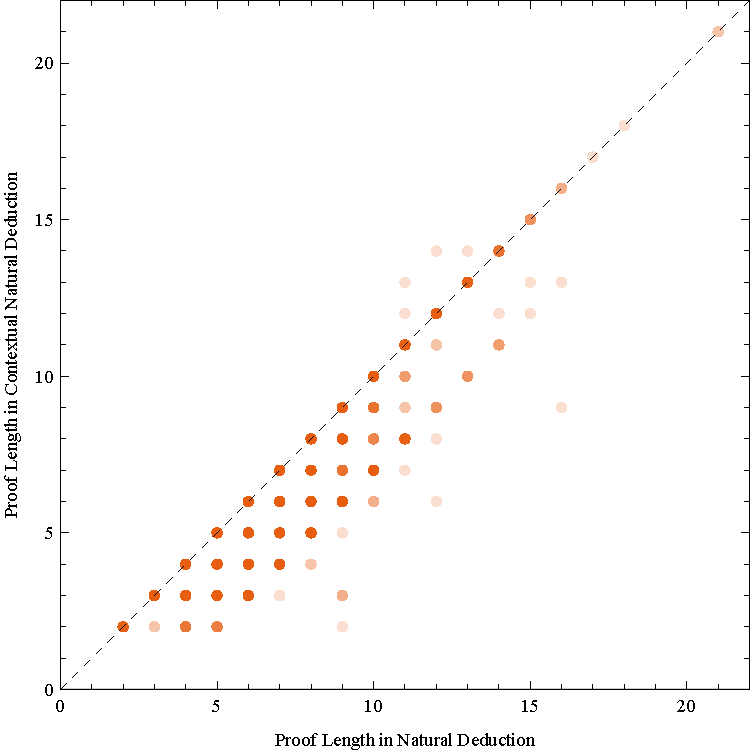
\includegraphics[width=0.8\textwidth]{Charts/Scatter.pdf}
        \caption{} \label{fig:Scatter}
\end{figure}

Among the 29594 formulas on which both provers were successful, 2557 (8.49\%) had shorter proofs in {\NDd} than in {\ND}. The total length of the {\NDd}-proofs was 2.97\% lesser than the total length of the proofs found by the {\ND} prover on all 29594 formulas. The total length of the {\NDd}-proofs was 27.8\% lesser than the total length of the {\ND}-proofs on the 2557 proofs that admit shorter {\NDd} proofs.

\begin{figure}[!ht]
        \centering
        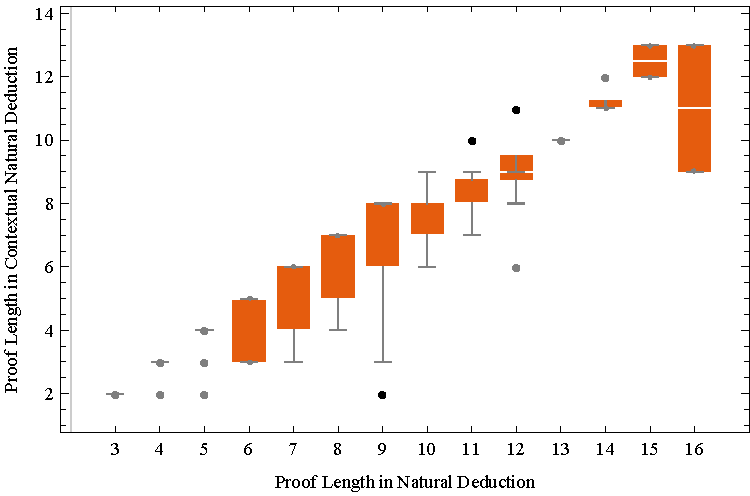
\includegraphics[width=0.8\textwidth]{Charts/BoxWhiskers.pdf}
        \caption{} \label{fig:BoxWhiskers}
\end{figure}


Figure \ref{fig:Time} (which takes into account all 76755 formulas) shows that the {\ND} prover rarely took longer than 10 milliseconds on a formula. The {\NDd} prover was, as expected, significantly slower than the {\ND} prover, because the search space for {\NDd} proofs is much larger. Nevertheless, the {\NDd} prover is surprinsingly faster in a few cases, probably due to the stricter upper-bound on proof height. 


\begin{figure}[!ht]
        \centering
        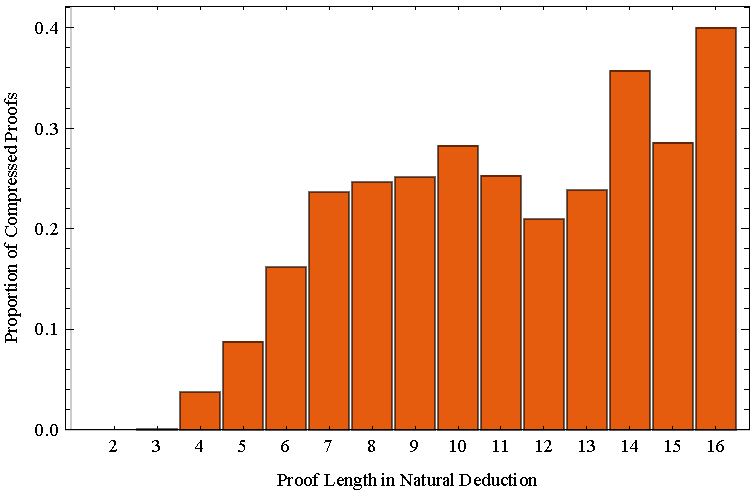
\includegraphics[width=0.8\textwidth]{Charts/ProportionByLength.pdf}
        \caption{ } \label{fig:ProportionByLength}
\end{figure}

\begin{figure}[!ht]
        \centering
        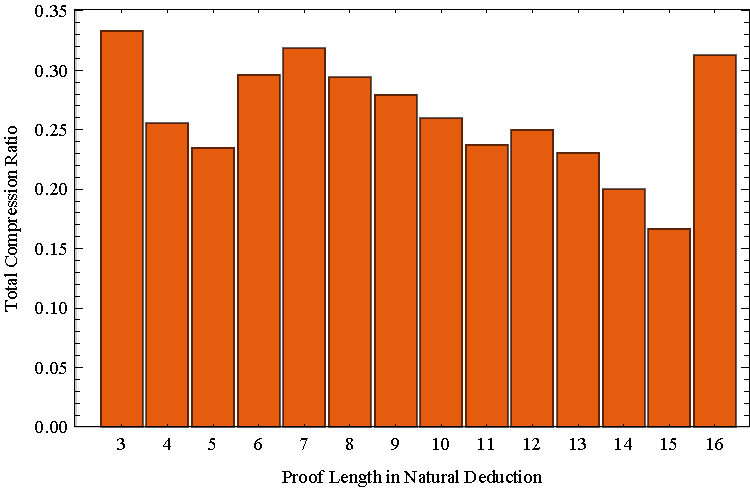
\includegraphics[width=0.8\textwidth]{Charts/CompressionByLength.pdf}
        \caption{ } \label{fig:CompressionByLength}
\end{figure}

\noindent
The 3D-charts in Figure \ref{fig:3D} shed further light on what influences the proportion of formulas that admit shorter {\NDd}-proofs and the total compression ratios (including all 29594 formulas). The proportion of formulas admitting shorter {\NDd}-proofs (and their total compression ratios) is higher the lower the number of distinct atoms they contain and the larger they are. The depths\footnote{$\mathrm{depth}(A) = 1$, for an atomic $A$; $\mathrm{depth}(B \imp C) = \mathrm{max}(\mathrm{depth}(B), \mathrm{depth}(C)) + 1$.} of the formulas also seem to play a role, with greater compression proportions and total compression ratios for intermediary depth values.

\begin{figure}[!ht]
  \centering
  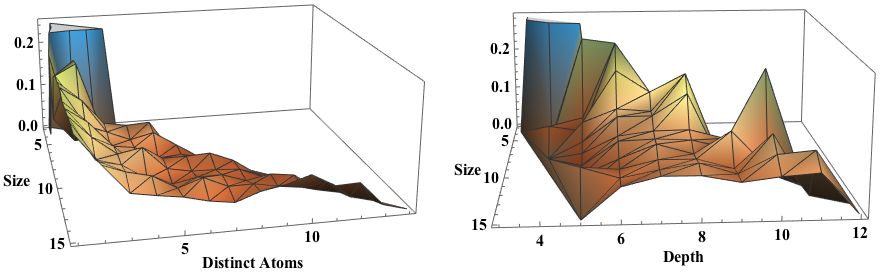
\includegraphics[width=\textwidth]{Charts/3DProportion.png}
  \caption{proportion of compressed proofs\\
           as a function of size, depth and distinct atoms\\
           in the formula being proven.} \label{fig:3D}
\end{figure}

\noindent
Figure \ref{fig:Time} (which takes into account all 76755 formulas) shows that the {\ND} prover rarely took longer than 10 milliseconds on a formula. Surprisingly, the {\NDd} prover was faster than the {\ND} prover in the majority of the cases (46733 formulas; 60.88\%), probably due to the stricter upper-bound on proof height. However, when the {\NDd} prover was slower, it tended to be significantly slower, as shown in the Figure. 

\begin{figure}[!ht]
        \centering
        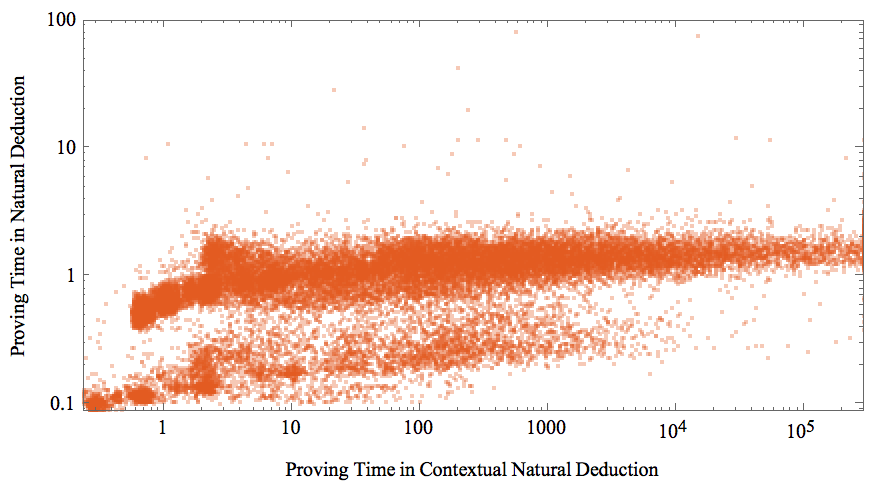
\includegraphics[width=0.8\textwidth]{Charts/Time.png}
        \caption{} \label{fig:Time}
\end{figure}


\section{Conclusions}

The empirical investigation reported in this paper confirms the expectation that {\NDd} can provide shorter proofs in a significant number of cases. Because the benchmarks were randomly generated, it is still an open question whether contextual natural deduction will perform well on real-world benchmarks. Nevertheless, the good performance on randomly generated benchmarks complements and the previous theoretical result of asymptotic best-case quadratic compression shown in \cite{NDc}. Together, the experimental evaluation and the theoretical improved proof complexity constitute strong evidence that contextualization is worth pursuing for the sake of obtaining shorter proofs in natural deduction style. 

The price to pay for shorter proofs is currently a much longer proving time. In this paper, proving time was restricted by bounding the proof height during proof search. Other more sophisticated techniques to restrict proof search should be investigated in the future, in order to improve the efficiency of theorem proving in {\NDd}.

To evaluate the benefit of contextual natural deduction on real-world benchmarks, it is firstly necessary to extend {\NDd} to the more expressive higher-order logics used by interactive proof assistants. Their libraries of formalized mathematics contain proofs of theorems for which shorter contextual natural deduction proofs could be possible. 


\bibliographystyle{plain}
\bibliography{Bibliography}



\end{document}
